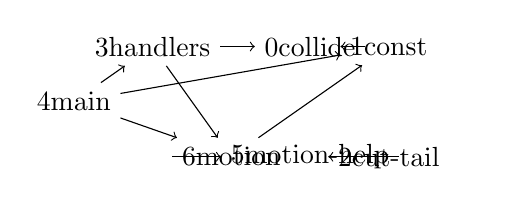
\begin{tikzpicture}

  \node (00)               {};
  \node (01) [below of=00,yshift=0.3cm] {};
  \node (02) [below of=01,yshift=0.3cm] {};

  \node (10) [left of=00] {\rkt{1}{const}};
  \node (11) [left of=01] {};
  \node (12) [left of=02] {\rkt{2}{cut-tail}};

  \node (20) [left of=10] {\rkt{0}{collide}};
  \node (21) [left of=11] {};
  \node (22) [left of=12] {\rkt{5}{motion-help}};

  \node (30) [left of=20] {};
  \node (31) [left of=21] {};
  \node (32) [left of=22] {\rkt{6}{motion}};

  \node (40) [left of=30] {\rkt{3}{handlers}};
  \node (41) [left of=31] {};
  \node (42) [left of=32] {};

  \node (51) [left of=41] {\rkt{4}{main}};

  %% -- edges
  %% collide
  \draw[->] (20) -- (10);
  %% motion-help
  \draw[->] (22) -- (12);
  %% motion
  \draw[->] (32) -- (10);
  \draw[->] (32) -- (22);
  %% handlers
  \draw[->] (40) -- (32);
  \draw[->] (40) -- (20);
  %% main
  \draw[->] (51) -- (10);
  \draw[->] (51) -- (40);
  \draw[->] (51) -- (32);
  
\end{tikzpicture}
